% answers.tex —— 1986 年·全国卷·文科 · 参考答案与详细解析片段
% 由 tools/generate_projects.py 依来源总账自 1986/1986_数学真题_全国文_试题.md + 1986/1986_数学真题_全国文_解析正文.md + 1986/1986_数学真题_全国文_答案要点.md 生成，勿手改（改源 MD 后重跑）


\begin{gktip}
固定源为一页题面，不含答案。以下逐题推导均为本库独立复算；第 10、17 题图形依据固定源重绘为 TikZ。
\end{gktip}

\begin{answer}
\gksolhead{1}{}

\textbf{题目}：

在下列各数中，已表示成三角形式的复数是\mbox{（　　）}

（A）$2\left(\cos\frac\pi4-i\sin\frac\pi4\right)$

（B）$2\left(\cos\frac\pi4+i\sin\frac\pi4\right)$

（C）$2\left(\sin\frac\pi4+i\cos\frac\pi4\right)$

（D）$-2\left(\sin\frac\pi4-i\cos\frac\pi4\right)$

\Needspace{4\baselineskip}
\textbf{解析}

复数的三角形式要求写成 $r(\cos\varphi+i\sin\varphi)$，其中 $r>0$。只有（B）直接符合这一形式，故选（B）。

\gkanswer{答案：B}

\end{answer}
\begin{answer}
\gksolhead{2}{}

\textbf{题目}：

\Needspace{5\baselineskip}
函数

\nopagebreak[4]
\[
y=5^x+1
\]

的反函数是\mbox{（　　）}

（A）$y=\log_5(x+1)$　　（B）$y=\log_x5+1$

（C）$y=\log_5(x-1)$　　（D）$y=\log_{x-1}5$

\Needspace{4\baselineskip}
\textbf{解析}

\Needspace{5\baselineskip}
由 $y=5^x+1$ 得 $x=\log_5(y-1)$，交换 $x\text{、}y$ 得反函数

\nopagebreak[4]
\[
y=\log_5(x-1).
\]

故选（C）。

\gkanswer{答案：C}

\end{answer}
\begin{answer}
\gksolhead{3}{}

\textbf{题目}：

已知全集 $I=\{1,2,3,4,5,6,7,8\}$，$A=\{3,4,5\}$，$B=\{1,3,6\}$，那么集合 $\{2,7,8\}$ 是\mbox{（　　）}

（A）$A\cup B$　　（B）$A\cap B$　　（C）$\overline A\cup\overline B$　　（D）$\overline A\cap\overline B$

\Needspace{4\baselineskip}
\textbf{解析}

\nopagebreak[4]
\[
\overline A=I\setminus A=\{1,2,6,7,8\},
\overline B=I\setminus B=\{2,4,5,7,8\}.
\]

\Needspace{5\baselineskip}
所以

\nopagebreak[4]
\[
\overline A\cap\overline B=\{2,7,8\}.
\]

故选（D）。

\gkanswer{答案：D}

\end{answer}
\begin{answer}
\gksolhead{4}{}

\textbf{题目}：

\Needspace{5\baselineskip}
函数

\nopagebreak[4]
\[
y=\sqrt2\sin2x\cos2x
\]

是\mbox{（　　）}

（A）周期为 $\dfrac\pi2$ 的奇函数　　（B）周期为 $\dfrac\pi2$ 的偶函数

（C）周期为 $\dfrac\pi4$ 的奇函数　　（D）周期为 $\dfrac\pi4$ 的偶函数

\Needspace{4\baselineskip}
\textbf{解析}

\nopagebreak[4]
\[
y=\sqrt2\sin2x\cos2x=\frac{\sqrt2}{2}\sin4x.
\]

其最小正周期为 $\pi/2$，且为奇函数，故选（A）。

\gkanswer{答案：A}

\end{answer}
\begin{answer}
\gksolhead{5}{}

\textbf{题目}：

已知 $c>0$，在下列不等式中成立的一个是\mbox{（　　）}

（A）$c>2^c$　　（B）$c>\left(\dfrac12\right)^c$

（C）$2^c<\left(\dfrac12\right)^c$　　（D）$2^c>\left(\dfrac12\right)^c$

\Needspace{4\baselineskip}
\textbf{解析}

\Needspace{5\baselineskip}
当 $c>0$ 时，底数大小关系 $2>\frac12$ 保持为幂的大小关系，因此

\nopagebreak[4]
\[
2^c>\left(\frac12\right)^c.
\]

故选（D）。

\gkanswer{答案：D}

\end{answer}
\begin{answer}
\gksolhead{6}{}

\textbf{题目}：

\Needspace{5\baselineskip}
有以下 20 个数：

\nopagebreak[4]
\[
87,\ 91,\ 94,\ 88,\ 93,\ 91,\ 89,\ 87,\ 92,\ 86,\ 90,\ 92,\ 88,\ 90,\ 91,
86,\ 89,\ 92,\ 95,\ 88,
\]

它们的和是\mbox{（　　）}

（A）1789　　（B）1799　　（C）1879　　（D）1899

\Needspace{4\baselineskip}
\textbf{解析}

\Needspace{5\baselineskip}
直接相加得

\nopagebreak[4]
\[
87+91+94+88+93+91+89+87+92+86
+90+92+88+90+91+86+89+92+95+88=1799.
\]

故选（B）。

\gkanswer{答案：B}

\end{answer}
\begin{answer}
\gksolhead{7}{}

\textbf{题目}：

已知某正方体对角线长为 $a$，那么这个正方体的全面积是\mbox{（　　）}

（A）$2\sqrt2a^2$　　（B）$2a^2$　　（C）$2\sqrt3a^2$　　（D）$3\sqrt2a^2$

\Needspace{4\baselineskip}
\textbf{解析}

\Needspace{5\baselineskip}
设正方体棱长为 $s$，则空间对角线满足 $a=\sqrt3s$。全面积为

\nopagebreak[4]
\[
6s^2=6\cdot\frac{a^2}{3}=2a^2.
\]

故选（B）。

\gkanswer{答案：B}

\end{answer}
\begin{answer}
\gksolhead{8}{}

\textbf{题目}：

\Needspace{5\baselineskip}
如果方程

\nopagebreak[4]
\[
x^2+y^2+Dx+Ey+F=0\ (D^2+E^2-4F>0)
\]

所表示的曲线关于直线 $y=x$ 对称，那么必有\mbox{（　　）}

（A）$D=E$　　（B）$D=F$　　（C）$E=F$　　（D）$D=E=F$

\Needspace{4\baselineskip}
\textbf{解析}

\Needspace{5\baselineskip}
将圆方程配方：

\nopagebreak[4]
\[
\left(x+\frac D2\right)^2+\left(y+\frac E2\right)^2
=\frac{D^2+E^2-4F}{4}.
\]

其圆心为 $\left(-\frac D2,-\frac E2\right)$。圆关于 $y=x$ 对称，当且仅当圆心在该直线上，所以 $D=E$，故选（A）。

\gkanswer{答案：A}

\end{answer}
\begin{answer}
\gksolhead{9}{}

\textbf{题目}：

设甲是乙的充分条件，乙是丙的充要条件，丙是丁的必要条件，那么丁是甲的\mbox{（　　）}

（A）充分条件　　（B）必要条件　　（C）充要条件　　（D）既不充分也不必要的条件

\Needspace{4\baselineskip}
\textbf{解析}

\Needspace{5\baselineskip}
把四个条件分别记为甲、乙、丙、丁，则

\nopagebreak[4]
\[
\text{\text{甲}}\Rightarrow\text{\text{乙}},
\text{\text{乙}}\Longleftrightarrow\text{\text{丙}},
\text{\text{丁}}\Rightarrow\text{\text{丙}}.
\]

这不能推出甲、丁之间的任一方向关系，因此丁是甲的既不充分也不必要条件，选（D）。

\gkanswer{答案：D}

\end{answer}
\begin{answer}
\gksolhead{10}{}

\textbf{题目}：

在下列各图中，$y=ax^2+bx$ 与 $y=ax+b$（$ab\ne0$）的图象只可能是\mbox{（　　）}
\nopagebreak[4]
\begin{center}% 1986 年全国卷文科第 10 题：四个函数图象选项
\begin{tikzpicture}[scale=0.72,>=stealth]
  \foreach \dx/\dy/\lab/\curve/\line in {
    0/2.25/{（A）}/{1.55*(\x+0.45)^2-0.55}/{0.85*\x+0.55},
    3.15/2.25/{（B）}/{1.55*\x*\x-1.55*\x}/{-0.85*\x+0.80},
    0/0/{（C）}/{-1.45*\x*\x+1.45*\x}/{-0.72*\x+0.85},
    3.15/0/{（D）}/{-1.45*\x*\x+1.45*\x}/{0.72*\x-0.55}
  } {
    \begin{scope}[shift={(\dx,\dy)}]
      \draw[->] (-1.35,0)--(1.45,0) node[right] {$x$};
      \draw[->] (0,-1.35)--(0,1.45) node[above] {$y$};
      \draw[thick,domain=-1.15:1.15,samples=80]
        plot (\x,{\curve});
      \draw[thick,domain=-1.25:1.25]
        plot (\x,{\line});
      \node[below] at (0,-1.65) {\lab};
      \node[below left] at (0,0) {$O$};
    \end{scope}
  }
\end{tikzpicture}
\end{center}
\nopagebreak[4]
\Needspace{4\baselineskip}
\textbf{解析}

\Needspace{5\baselineskip}
抛物线和直线的交点横坐标满足

\nopagebreak[4]
\[
ax^2+bx=ax+b,
\]

\Needspace{5\baselineskip}
即

\nopagebreak[4]
\[
(x-1)(ax+b)=0.
\]

\Needspace{5\baselineskip}
另一方面，抛物线

\nopagebreak[4]
\[
y=x(ax+b)
\]

必过原点，并在 $x=-b/a$ 处与 $x$ 轴相交；直线也在该点通过。再结合直线斜率为 $a$ 与抛物线开口方向由 $a$ 决定，四图中只有（C）相容。

\gkanswer{答案：C}

\end{answer}
\begin{answer}
\gksolhead{11}{}

\textbf{题目}：

\Needspace{5\baselineskip}
求方程

\nopagebreak[4]
\[
\sqrt{25^{x^2+x-0.5}}=\sqrt[4]{5}
\]

的解。

\Needspace{4\baselineskip}
\textbf{解析}

\Needspace{5\baselineskip}
令 $t=x^2+x-\frac12$，则

\nopagebreak[4]
\[
\sqrt{25^t}=5^t,\ \sqrt[4]{5}=5^{1/4}.
\]

\Needspace{5\baselineskip}
所以

\nopagebreak[4]
\[
x^2+x-\frac12=\frac14,
\]

\Needspace{5\baselineskip}
即

\nopagebreak[4]
\[
x^2+x-\frac34=0.
\]

\Needspace{5\baselineskip}
故

\nopagebreak[4]
\[
x=\frac12\ \text{\text{或}}\ x=-\frac32.
\]

\gkanswer{答案：$x=\dfrac12$ 或 $x=-\dfrac32$。}

\end{answer}
\begin{answer}
\gksolhead{12}{}

\textbf{题目}：

\Needspace{5\baselineskip}
已知

\nopagebreak[4]
\[
\omega=\frac{-1-\sqrt3i}{2},
\]

求 $\omega^2+\omega+1$ 的值。

\Needspace{4\baselineskip}
\textbf{解析}

\nopagebreak[4]
\[
\omega=-\frac12-\frac{\sqrt3}{2}i
\]

是非实三次单位根，满足 $\omega^2+\omega+1=0$，故所求值为 $0$。

\gkanswer{答案：$0$。}

\end{answer}
\begin{answer}
\gksolhead{13}{}

\textbf{题目}：

在 $xOy$ 平面上，$\triangle ABC$ 的三个顶点坐标依次为 $(0,0)$、$(1,0)$、$(0,3)$，将这个三角形绕 $x$ 轴旋转一周，求所得到的几何体的体积。

\Needspace{4\baselineskip}
\textbf{解析}

\Needspace{5\baselineskip}
三角形绕 $x$ 轴旋转后是底面半径为 $3$、高为 $1$ 的圆锥，故

\nopagebreak[4]
\[
V=\frac13\pi\cdot3^2\cdot1=3\pi.
\]

\gkanswer{答案：$3\pi$。}

\end{answer}
\begin{answer}
\gksolhead{14}{}

\textbf{题目}：

\Needspace{5\baselineskip}
求

\nopagebreak[4]
\[
\lim_{n\to\infty}\frac{2n^2+n+7}{5n^2+4}.
\]

\Needspace{4\baselineskip}
\textbf{解析}

\Needspace{5\baselineskip}
同除以 $n^2$：

\nopagebreak[4]
\[
\lim_{n\to\infty}
\frac{2+\frac1n+\frac7{n^2}}{5+\frac4{n^2}}
=\frac25.
\]

\gkanswer{答案：$\dfrac25$。}

\end{answer}
\begin{answer}
\gksolhead{15}{}

\textbf{题目}：

\Needspace{5\baselineskip}
求

\nopagebreak[4]
\[
\left(2x^3-\frac1{x^2}\right)^5
\]

展开式中的常数项。

\Needspace{4\baselineskip}
\textbf{解析}

\Needspace{5\baselineskip}
通项

\nopagebreak[4]
\[
\binom5k(2x^3)^{5-k}\left(-\frac1{x^2}\right)^k
\]

\Needspace{5\baselineskip}
中的幂次为 $15-5k$。常数项要求 $k=3$，所以常数项为

\nopagebreak[4]
\[
\binom53 2^2(-1)^3=-40.
\]

\gkanswer{答案：$-40$。}

\end{answer}
\begin{answer}
\gksolhead{16}{}

\textbf{题目}：

\Needspace{5\baselineskip}
求与椭圆

\nopagebreak[4]
\[
\frac{x^2}{9}+\frac{y^2}{4}=1
\]

有公共焦点，且离心率为 $\dfrac{\sqrt5}{2}$ 的双曲线方程。

\Needspace{4\baselineskip}
\textbf{解析}

\Needspace{5\baselineskip}
椭圆的焦距参数为

\nopagebreak[4]
\[
c=\sqrt{3^2-2^2}=\sqrt5.
\]

\Needspace{5\baselineskip}
设所求双曲线为 $\frac{x^2}{a^2}-\frac{y^2}{b^2}=1$。公共焦点给出 $c=\sqrt5$，离心率条件

\nopagebreak[4]
\[
\frac ca=\frac{\sqrt5}{2}
\]

\Needspace{5\baselineskip}
给出 $a=2$。再由 $c^2=a^2+b^2$ 得 $b^2=1$，故

\nopagebreak[4]
\[
\frac{x^2}{4}-y^2=1.
\]

\gkanswer{答案：$\dfrac{x^2}{4}-y^2=1$。}

\end{answer}
\begin{answer}
\gksolhead{17}{}

\textbf{题目}：

如图，$AB$ 是圆 $O$ 的直径，$PA$ 垂直于圆 $O$ 所在的平面，$C$ 是圆周上不同于 $A\text{、}B$ 的任一点，求证：平面 $PAC$ 垂直于平面 $PBC$。
\nopagebreak[4]
\begin{center}% 1986 年全国卷文科第 17 题：圆的直径与三棱锥示意图
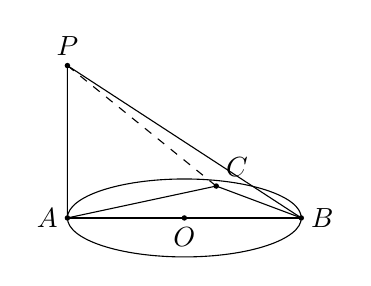
\begin{tikzpicture}[scale=0.9,>=stealth]
  \draw (0,0) ellipse (1.65 and 0.55);
  \draw[dashed] (-1.65,0)--(1.65,0);
  \draw (-1.65,0)--(1.65,0);
  \fill (0,0) circle (1.1pt) node[below] {$O$};
  \fill (-1.65,0) circle (1.1pt) node[left] {$A$};
  \fill (1.65,0) circle (1.1pt) node[right] {$B$};
  \coordinate (C) at (0.45,0.45);
  \fill (C) circle (1.1pt) node[above right] {$C$};
  \coordinate (P) at (-1.65,2.15);
  \fill (P) circle (1.1pt) node[above] {$P$};
  \draw (P)--(-1.65,0);
  \draw (P)--(1.65,0);
  \draw[dashed] (P)--(C);
  \draw (C)--(-1.65,0);
  \draw (C)--(1.65,0);
\end{tikzpicture}
\end{center}
\nopagebreak[4]
\Needspace{4\baselineskip}
\textbf{解析}

\Needspace{5\baselineskip}
因为 $AB$ 是圆的直径，所以由圆周角定理

\nopagebreak[4]
\[
\angle ACB=90^\circ,\ AC\perp BC.
\]

\Needspace{5\baselineskip}
又因 $PA$ 垂直于圆所在平面，且 $BC$ 在该平面内，所以 $PA\perp BC$。直线 $PA\text{、}AC$ 是平面 $PAC$ 内相交的两条直线，$BC$ 同时垂直于它们，故

\nopagebreak[4]
\[
BC\perp\text{\text{平面} }PAC.
\]

\Needspace{5\baselineskip}
而 $BC$ 在平面 $PBC$ 内，所以

\nopagebreak[4]
\[
\text{\text{平面} }PAC\perp\text{\text{平面} }PBC.
\]

\gkanswer{答案：$\text{\text{平面} }PAC\perp\text{\text{平面} }PBC$。}

\end{answer}
\begin{answer}
\gksolhead{18}{}

\textbf{题目}：

\Needspace{5\baselineskip}
求满足方程

\nopagebreak[4]
\[
|z+3-\sqrt3i|=\sqrt3
\]

的辐角主值最小的复数 $z$。

\Needspace{4\baselineskip}
\textbf{解析}

\Needspace{5\baselineskip}
复数方程表示圆

\nopagebreak[4]
\[
\left|z-(-3+\sqrt3i)\right|=\sqrt3,
\]

\Needspace{5\baselineskip}
其圆心到原点的距离为 $2\sqrt3$，圆心辐角为 $5\pi/6$。从原点向圆作切线，切线半角满足

\nopagebreak[4]
\[
\sin\alpha=\frac{\sqrt3}{2\sqrt3}=\frac12,
\alpha=\frac\pi6.
\]

\Needspace{5\baselineskip}
两条切线的辐角主值为 $2\pi/3$ 与 $\pi$，最小者为 $2\pi/3$。对应切点到原点距离为

\nopagebreak[4]
\[
\sqrt{(2\sqrt3)^2-(\sqrt3)^2}=3,
\]

\Needspace{5\baselineskip}
故

\nopagebreak[4]
\[
z=3\left(\cos\frac{2\pi}{3}+i\sin\frac{2\pi}{3}\right)
=-\frac32+\frac{3\sqrt3}{2}i.
\]

\gkanswer{答案：$z=-\dfrac32+\dfrac{3\sqrt3}{2}i$，其辐角主值为 $\dfrac{2\pi}{3}$。}

\end{answer}
\begin{answer}
\gksolhead{19}{}

\textbf{题目}：

\Needspace{5\baselineskip}
已知抛物线

\nopagebreak[4]
\[
y^2=x+1,
\]

定点 $A(3,1)$，$B$ 为抛物线上任意一点，点 $P$ 在线段 $AB$ 上，且有 $BP:PA=1:2$。当点 $B$ 在抛物线上变动时，求点 $P$ 的轨迹方程，并指出这个轨迹为哪种曲线。

\Needspace{4\baselineskip}
\textbf{解析}

\Needspace{5\baselineskip}
设 $B=(X,Y)$，则 $Y^2=X+1$。由 $BP:PA=1:2$，内分公式得

\nopagebreak[4]
\[
P=\frac{A+2B}{3},
\]

\Needspace{5\baselineskip}
即

\nopagebreak[4]
\[
x=\frac{3+2X}{3},\ y=\frac{1+2Y}{3}.
\]

\Needspace{5\baselineskip}
代入 $X=Y^2-1$：

\nopagebreak[4]
\[
x=\frac{2Y^2+1}{3},\ y=\frac{2Y+1}{3}.
\]

\Needspace{5\baselineskip}
消去 $Y$ 得

\nopagebreak[4]
\[
6x=(3y-1)^2+2,
\]

\Needspace{5\baselineskip}
即

\nopagebreak[4]
\[
3y^2-2y-2x+1=0.
\]

这是顶点为 $\left(\frac13,\frac13\right)$、开口向右的抛物线。

\gkanswer{答案：$3y^2-2y-2x+1=0$，即 $\left(y-\dfrac13\right)^2=\dfrac23\left(x-\dfrac13\right)$，是开口向右的抛物线。}

\end{answer}
\begin{answer}
\gksolhead{20}{}

\textbf{题目}：

甲、乙、丙、丁四个公司承包 8 项工程，甲公司承包 3 项，乙公司承包 1 项，丙、丁两个公司各承包 2 项，问共有多少种承包方式。

\Needspace{4\baselineskip}
\textbf{解析}

\Needspace{5\baselineskip}
8 项不同的工程按甲、乙、丙、丁分配，方式数为

\nopagebreak[4]
\[
\frac{8!}{3!\,1!\,2!\,2!}=1680.
\]

\gkanswer{答案：$1680$。}

\end{answer}
\begin{answer}
\gksolhead{21}{}

\textbf{题目}：

\Needspace{5\baselineskip}
已知

\nopagebreak[4]
\[
\sin A+\sin3A+\sin5A=a,
\cos A+\cos3A+\cos5A=b.
\]

求证：

（1） 当 $b\ne0$ 时，$\tan3A=\dfrac ab$；

（2） $(1+2\cos2A)^2=a^2+b^2$。

\Needspace{4\baselineskip}
\textbf{解析}

\gksubpart{（1）}

\Needspace{5\baselineskip}
由和差化积，

\nopagebreak[4]
\[
\sin A+\sin5A=2\sin3A\cos2A,
\]

\Needspace{5\baselineskip}
所以

\nopagebreak[4]
\[
a=\sin3A(1+2\cos2A).
\]

\Needspace{5\baselineskip}
同理，

\nopagebreak[4]
\[
b=\cos3A(1+2\cos2A).
\]

\Needspace{5\baselineskip}
当 $b\ne0$ 时，

\nopagebreak[4]
\[
\frac ab=\tan3A.
\]

\gksubpart{（2）}

\Needspace{5\baselineskip}
另外，

\nopagebreak[4]
\[
\begin{aligned}
a^2+b^2
&=(1+2\cos2A)^2(\sin^23A+\cos^23A)\\
&=(1+2\cos2A)^2.
\end{aligned}
\]

\gkanswer{答案（1）：$\tan3A=\dfrac ab$。}

\gkanswer{答案（2）：$(1+2\cos2A)^2=a^2+b^2$。}

\end{answer}
\begin{answer}
\gksolhead{22}{}

\textbf{题目}：

\Needspace{5\baselineskip}
已知数列 $\{a_n\}$，其中

\nopagebreak[4]
\[
a_1=\frac43,\ a_2=\frac{13}{9},
\]

\Needspace{5\baselineskip}
且当 $n\ge3$ 时，

\nopagebreak[4]
\[
a_n-a_{n-1}=\frac13(a_{n-1}-a_{n-2}).
\]

（1） 求数列 $\{a_n\}$ 的通项公式；

（2） 求 $\displaystyle\lim_{n\to\infty}a_n$。

\Needspace{4\baselineskip}
\textbf{解析}

\gksubpart{（1）}

\Needspace{5\baselineskip}
令 $d_n=a_n-a_{n-1}$（$n\ge2$），则

\nopagebreak[4]
\[
d_2=\frac{13}{9}-\frac43=\frac19,
d_n=\frac13d_{n-1}.
\]

\Needspace{5\baselineskip}
因此

\nopagebreak[4]
\[
d_n=\frac19\left(\frac13\right)^{n-2}.
\]

\Needspace{5\baselineskip}
从而

\nopagebreak[4]
\[
\begin{aligned}
a_n
&=\frac43+\sum_{k=2}^n d_k\\
&=\frac43+\frac16\left(1-\frac1{3^{n-1}}\right)\\
&=\frac32-\frac{1}{2\cdot3^n}.
\end{aligned}
\]

\gksubpart{（2）}

\Needspace{5\baselineskip}
所以

\nopagebreak[4]
\[
\lim_{n\to\infty}a_n=\frac32.
\]

\gkanswer{答案（1）：$a_n=\dfrac32-\dfrac{1}{2\cdot3^n}$。}

\gkanswer{答案（2）：$\displaystyle\lim_{n\to\infty}a_n=\dfrac32$。}

\end{answer}